%==========================================================================
%Template File
%   Copyright (C) 2006-2009                                
%           by Shinya Watanabe(sin@csse.muroran-it.ac.jp) 
%==========================================================================
\documentclass[a4j,titlepage]{jarticle}
\usepackage{programing_report}

\begin{document}

%--------------------
%以下に実験レポートのタイトル,自分のクラス名,学籍番号,氏名,提出日を書く.
%--------------------

%%\title{レポートタイトル}を記述する.
\title{第X回 プログラミング演習 レポート}

%%\author{クラス名}{学籍番号}{氏名}を記述する.
\author{123456789-0○○○○}{室蘭 情報}

%%\date{提出する年月日}を記述する.
\date{20xx 年 x 月x 日}
\maketitle

%--------------------
%以下から本文を開始する.
%--------------------

\section{はじめに}

本レポートでは,\TeX を使用したレポート作成方法の概略について説明する.使用しているスタイルファイル
(programing\_\!report)は実験レポートのためのスタイルオプションファイルである.

本レポートのようにスタイルファイルを使用する場合,参照する\TeX ファイルと同じディレクトリもしくは\TeX コンパイラの参照パスが通っている場所(\verb|c:/tex/share/texmf/ptex/platex/base/| , デフォルトでインストールした場合のフォルダ)に使用するスタイルファイルを置いておく必要がある.

ここでは\TeX に関する詳細(コマンド, 環境など)ついては,一切ふれない.\TeX に関する詳細は,奥村さんの書籍~\cite{okumura}, \TeX Wiki~\cite{tex-wiki}, 乙部さんの書籍~\cite{otobe}などを参考に各自勉強すること.また,Windowsでの\TeX インストールに関しては,\url{http://is.csse.muroran-it.ac.jp/~sin/lecture/}~\cite{watanbe-ulr}を参照すること.


以下,下記の事柄について説明する.
\begin{itemize}
\item 演習レポートの書き方
\item プログラムソースの載せ方
\item プログラム実行例の載せ方
\item 図表の書き方,参照方法
\item 式の書き方,参照方法
\end{itemize}

\section{演習レポートの書き方}
演習レポートには,作成したプログラムソース,実行例,考察を必ず載せること(考察不要の場合には省略して構わない).プログラムソースは,他者が読んでも内容が理解できるようコメント,インデントに配慮して作成する必要がある.また,考察では得られた実行結果から読み取れる内容について論理的に分かりやすく記述し自分なりに分析した事柄について説明すること.

\section{プログラムソースの貼り方}
プログラムソース中には\TeX における特殊記号が多数含まれるため,一般にはverbatim環境を利用する.
一例を下記に示す.

\begin{itembox}[l]{Hello world} \small
\begin{verbatim}
/********************************************
名前: hello.c
機能: ウェルカムメッセージを表示する
入力: なし
出力: なし
作者: (自分の学籍番号と名前)
制作日: 2008/10/15
特記事項: 特になし
********************************************/

#include <stdio.h>

int main( void )
{
    printf("ようこそC言語の世界へ!");
    printf("ようこそC言語の世界へ!\n");
    printf("ようこそ\n C言語の世界へ!\n");
	
    return 0;
}
\end{verbatim}
\end{itembox}

\section{プログラムの実行例の載せ方}
プログラムの実行に関しても,ソースの場合と同様\TeX における特殊記号の影響を避けるためverbatim環境を利用する.下記に一例を示す.

\begin{itembox}[l]{コンパイルと実行}
\begin{verbatim}
$ gcc -o hello hello.c
$ ./hello
ようこそC言語の世界へ!ようこそC言語の世界へ!
ようこそ
C言語の世界へ!
\end{verbatim}
\end{itembox}

\section{図表の書き方}

\subsection{図について}

図を出力するためには,下記のような書式で記述する.

\begin{screen}
\begin{verbatim}
\begin{figure}[htbp]
\begin{center}
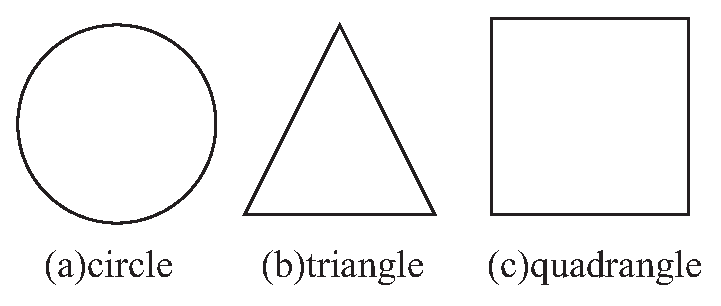
\includegraphics[width=0.7\linewidth]{eps/graphic_data.eps}
\end{center}
\caption{図形}
\label{fig::graphic}
\end{figure}
\end{verbatim}
\end{screen}

\begin{figure}[htbp]
\begin{center}
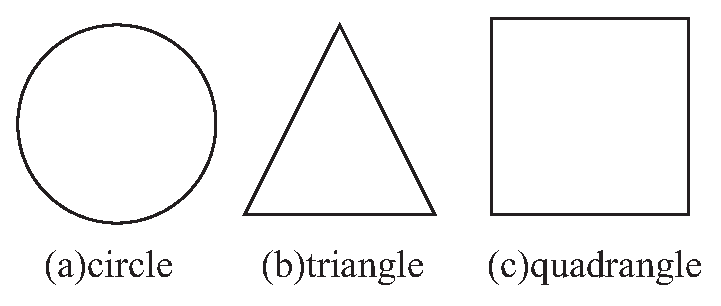
\includegraphics[width=0.7\linewidth]{eps/graphic_data.eps}
\end{center}
\caption{図形}
\label{fig::graphic}
\end{figure}

\verb|\begin{figure}[htbp]|における[htbp]は図を文章のなかに入れ込む位置に関するパラメータであり,Here(この場所で),Top(ページの上で),Bottom(ページの下で),Page(次のページにおいて)の頭文字を意味する.論文などにおいて,図はページの上もしくは下に挿入することが一般的であるためオプションとしては,\verb|\begin{figure}[tbp]|を勧める.

また,\verb|\label{ラベル名}|はこの図形を自動参照するためのラベル付けである.図を参照する場合には,このラベルを参照して\verb|\fgref{ラベル名}|と記述する\footnote{fgref は,Figure(図形)のReference(参照)を意味する.}.この場合の例では,\verb|\fgref{fig::graphic}|と記述することにより,「\fgref{fig::graphic}」となる.

なお,図におけるキャプションは{\bf 必ず図の下}につけること.

\subsection{表について}

表を出力するためには,下記のような書式で記述する.

\begin{screen}
\begin{verbatim}
\begin{table}[tbp]
\begin{center}
\caption{Problem Instance.}
\label{tb::example}
\begin{tabular}{ccccc}
\hline 
Problem & $N$ & $W$ & $\bar{w}$ & $\sigma (w)$\\
\hline \hline
tai75a & 75 & 1445 & 183.4 & 242.9\\
tai75b & 75 & 1679 & 198.7 &  273.4\\
tai100a & 100 & 1409 & 152.0 &  201.5\\
tai150a & 150 & 1544 & 145.54 & 200.7\\
\hline
\end{tabular}
\end{center}
\end{table}
\end{verbatim}
\end{screen}

\begin{table}[tbp]
\begin{center}
\caption{Problem Instance.}
\label{tb::example}
\begin{tabular}{c|cccc}
\hline 
Problem & $N$ & $W$ & $\bar{w}$ & $\sigma (w)$\\
\hline \hline
tai75a & 75 & 1445 & 183.4 & 242.9\\
tai75b & 75 & 1679 & 198.7 &  273.4\\
tai100a & 100 & 1409 & 152.0 &  201.5\\
tai150a & 150 & 1544 & 145.54 & 200.7\\
\hline
\end{tabular}
\end{center}
\end{table}


基本的には,図における場合と同様に\verb|\begin{table}[htbp]|により表の文中での位置を決め,\verb|\label{ラベル名}|で表のラベル付けを行う.
また,表を参照する際には\verb|\tbref{ラベル名}|と記述する\footnote{tbref は,Table(表)のReference(参照)を意味する.}.この場合の例では,\verb|\tbref{tb::example}|と記述することにより,「\tbref{tb::example}」となる.

なお,表におけるキャプションは{\bf 必ず表の上}につけること.

\section{式について}

式の書き方には幾つかの種類がある.以下,それぞれについて示す.
\begin{enumerate}
\item 文中で式を入れ込む場合\\
 \verb|$数式$|という書き方をする.例えば,\verb|$\cfrac{b_{2}}{a^2}\le 0$|と記述すると,「$\cfrac{b_{2}}{a^2}\le 0$」のように出力される.
\item 数式を番号なしで1行挿入する場合\\
 \verb| \[ \] |と記述する.\\
例えば,
\verb| \[ \cfrac{b_{2}}{a^2}\le 0 \]|と記述すると,下記のように出力される.
\[ \cfrac{b_{2}}{a^2}\le 0 \]
\item 数式を番号つきで1行挿入する場合\\
\verb| \begin{equation} 式 \end{equation}|と記述する.\\
例えば,\verb| \begin{equation} \cfrac{b_{2}}{a^2}\le 0 \end{equation}|と記述すると,下記のように出力される.
\begin{equation} \cfrac{b_{2}}{a^2}\le 0 \end{equation}
\item 数式を番号なしで複数行挿入する場合\\
\verb| \begin{eqnarray*} 式1 \\ 式2  \end{eqnarray*}|と記述する.\\
例えば,\verb| \begin{eqnarray*} \cfrac{b_{2}}{a^2}\le 0 \\ a\times b \ge 10  \end{eqnarray*}|と記述すると,下記のように出力される.
\begin{eqnarray*} \cfrac{b_{2}}{a^2}\le 0 \\ a\times b \ge 10  \end{eqnarray*}
\item 数式を番号つきで複数行挿入する場合\\
\verb| \begin{eqnarray} 式1 \\ 式2  \end{eqnarray}|と記述する.\\
例えば,\verb| \begin{eqnarray} \cfrac{b_{2}}{a^2}\le 0 \\ a\times b \ge 10  \end{eqnarray}|と記述すると,下記のように出力される.
\begin{eqnarray} \cfrac{b_{2}}{a^2}\le 0 \\ a\times b \ge 10  \end{eqnarray}
\end{enumerate}

なお,番号付きの式には図,表と同様にラベル付けおよびその参照を行うことができる.一例を以下に示す.

\begin{screen}
\begin{verbatim}
\begin{eqnarray} 
\cfrac{b_{2}}{a^2}\le 0  \label{eq::const-1} \\
a\times b \ge 10  \label{eq::const-2} 
\end{eqnarray}
\end{verbatim}
\end{screen}


\begin{eqnarray} 
\cfrac{b_{2}}{a^2}\le 0  \label{eq::const-1} \\
a\times b \ge 10  \label{eq::const-2} 
\end{eqnarray}

式を参照するときには,\verb|\eqref{式ラベル}|と記述する.上記の例では\verb|\eqref{eq::const-1}|と記述することにより「\eqref{eq::const-1}」が出力される.

ちなみに図,表,式だけでなく章(section),節(subsection)など様々な箇所でラベル付けおよびその参照を行うことができる.その場合には,\verb|\ref{ラベル}|と記述することによってラベル付けされた場所の番号を呼び出すことができる.そのため,たとえば章の場合,\verb|\ref{ラベル}章|といった書き方を行うことになる.

%------------
%以下,参考文献に関する記述
%------------
\begin{thebibliography}{9}
\small{
\bibitem{okumura} 奥村 「LATEX2ε 美文書作成入門」技術評論社, 2000年
\bibitem{tex-wiki} TeX Wiki \newblock \url{http://cise.edu.mie-u.ac.jp/%7eokumura/texwiki/}
\bibitem{otobe} 乙部厳己・江口庄英 「pLaTeX2e for Windows Another Manual Vol.1 Basic Kit 1999」 ソフトバンクパブリッシング, 1999年
\bibitem{watanbe-ulr}  TeXを使用したレポート作成に関するHP \newblock \url{http://is.csse.muroran-it.ac.jp/~sin/lecture/}
}
\end{thebibliography}
\end{document}
